
%% bare_conf.tex
%% V1.3
%% 2007/01/11
%% by Michael Shell
%% See:
%% http://www.michaelshell.org/
%% for current contact information.
%%
%% This is a skeleton file demonstrating the use of IEEEtran.cls
%% (requires IEEEtran.cls version 1.7 or later) with an IEEE conference paper.
%%
%% Support sites:
%% http://www.michaelshell.org/tex/ieeetran/
%% http://www.ctan.org/tex-archive/macros/latex/contrib/IEEEtran/
%% and
%% http://www.ieee.org/

%%*************************************************************************
%% Legal Notice:
%% This code is offered as-is without any warranty either expressed or
%% implied; without even the implied warranty of MERCHANTABILITY or
%% FITNESS FOR A PARTICULAR PURPOSE! 
%% User assumes all risk.
%% In no event shall IEEE or any contributor to this code be liable for
%% any damages or losses, including, but not limited to, incidental,
%% consequential, or any other damages, resulting from the use or misuse
%% of any information contained here.
%%
%% All comments are the opinions of their respective authors and are not
%% necessarily endorsed by the IEEE.
%%
%% This work is distributed under the LaTeX Project Public License (LPPL)
%% ( http://www.latex-project.org/ ) version 1.3, and may be freely used,
%% distributed and modified. A copy of the LPPL, version 1.3, is included
%% in the base LaTeX documentation of all distributions of LaTeX released
%% 2003/12/01 or later.
%% Retain all contribution notices and credits.
%% ** Modified files should be clearly indicated as such, including  **
%% ** renaming them and changing author support contact information. **
%%
%% File list of work: IEEEtran.cls, IEEEtran_HOWTO.pdf, bare_adv.tex,
%%                    bare_conf.tex, bare_jrnl.tex, bare_jrnl_compsoc.tex
%%*************************************************************************

% *** Authors should verify (and, if needed, correct) their LaTeX system  ***
% *** with the testflow diagnostic prior to trusting their LaTeX platform ***
% *** with production work. IEEE's font choices can trigger bugs that do  ***
% *** not appear when using other class files.                            ***
% The testflow support page is at:
% http://www.michaelshell.org/tex/testflow/



% Note that the a4paper option is mainly intended so that authors in
% countries using A4 can easily print to A4 and see how their papers will
% look in print - the typesetting of the document will not typically be
% affected with changes in paper size (but the bottom and side margins will).
% Use the testflow package mentioned above to verify correct handling of
% both paper sizes by the user's LaTeX system.
%
% Also note that the "draftcls" or "draftclsnofoot", not "draft", option
% should be used if it is desired that the figures are to be displayed in
% draft mode.
%
\documentclass[conference]{IEEEtran}
%% INFOCOM 2013 addition:
\makeatletter
\def\ps@headings{%
\def\@oddhead{\mbox{}\scriptsize\rightmark \hfil \thepage}%
\def\@evenhead{\scriptsize\thepage \hfil \leftmark\mbox{}}%
\def\@oddfoot{}%
\def\@evenfoot{}}
\makeatother
\pagestyle{headings}
% Add the compsoc option for Computer Society conferences.
%
% If IEEEtran.cls has not been installed into the LaTeX system files,
% manually specify the path to it like:
% \documentclass[conference]{../sty/IEEEtran}





% Some very useful LaTeX packages include:
% (uncomment the ones you want to load)


% *** MISC UTILITY PACKAGES ***
%
%\usepackage{ifpdf}
% Heiko Oberdiek's ifpdf.sty is very useful if you need conditional
% compilation based on whether the output is pdf or dvi.
% usage:
% \ifpdf
%   % pdf code
% \else
%   % dvi code
% \fi
% The latest version of ifpdf.sty can be obtained from:
% http://www.ctan.org/tex-archive/macros/latex/contrib/oberdiek/
% Also, note that IEEEtran.cls V1.7 and later provides a builtin
% \ifCLASSINFOpdf conditional that works the same way.
% When switching from latex to pdflatex and vice-versa, the compiler may
% have to be run twice to clear warning/error messages.






% *** CITATION PACKAGES ***
%
\usepackage{cite}
% cite.sty was written by Donald Arseneau
% V1.6 and later of IEEEtran pre-defines the format of the cite.sty package
% \cite{} output to follow that of IEEE. Loading the cite package will
% result in citation numbers being automatically sorted and properly
% "compressed/ranged". e.g., [1], [9], [2], [7], [5], [6] without using
% cite.sty will become [1], [2], [5]--[7], [9] using cite.sty. cite.sty's
% \cite will automatically add leading space, if needed. Use cite.sty's
% noadjust option (cite.sty V3.8 and later) if you want to turn this off.
% cite.sty is already installed on most LaTeX systems. Be sure and use
% version 4.0 (2003-05-27) and later if using hyperref.sty. cite.sty does
% not currently provide for hyperlinked citations.
% The latest version can be obtained at:
% http://www.ctan.org/tex-archive/macros/latex/contrib/cite/
% The documentation is contained in the cite.sty file itself.






% *** GRAPHICS RELATED PACKAGES ***
%
\ifCLASSINFOpdf
  \usepackage[pdftex]{graphicx}
  % declare the path(s) where your graphic files are
  \graphicspath{{./eps/}}
  % and their extensions so you won't have to specify these with
  % every instance of \includegraphics
  \DeclareGraphicsExtensions{.pdf,.jpeg,.png}
\else
  % or other class option (dvipsone, dvipdf, if not using dvips). graphicx
  % will default to the driver specified in the system graphics.cfg if no
  % driver is specified.
  % \usepackage[dvips]{graphicx}
  % declare the path(s) where your graphic files are
  % \graphicspath{{../eps/}}
  % and their extensions so you won't have to specify these with
  % every instance of \includegraphics
  % \DeclareGraphicsExtensions{.eps}
\fi
% graphicx was written by David Carlisle and Sebastian Rahtz. It is
% required if you want graphics, photos, etc. graphicx.sty is already
% installed on most LaTeX systems. The latest version and documentation can
% be obtained at: 
% http://www.ctan.org/tex-archive/macros/latex/required/graphics/
% Another good source of documentation is "Using Imported Graphics in
% LaTeX2e" by Keith Reckdahl which can be found as epslatex.ps or
% epslatex.pdf at: http://www.ctan.org/tex-archive/info/
%
% latex, and pdflatex in dvi mode, support graphics in encapsulated
% postscript (.eps) format. pdflatex in pdf mode supports graphics
% in .pdf, .jpeg, .png and .mps (metapost) formats. Users should ensure
% that all non-photo figures use a vector format (.eps, .pdf, .mps) and
% not a bitmapped formats (.jpeg, .png). IEEE frowns on bitmapped formats
% which can result in "jaggedy"/blurry rendering of lines and letters as
% well as large increases in file sizes.
%
% You can find documentation about the pdfTeX application at:
% http://www.tug.org/applications/pdftex





% *** MATH PACKAGES ***
%
%\usepackage[cmex10]{amsmath}
% A popular package from the American Mathematical Society that provides
% many useful and powerful commands for dealing with mathematics. If using
% it, be sure to load this package with the cmex10 option to ensure that
% only type 1 fonts will utilized at all point sizes. Without this option,
% it is possible that some math symbols, particularly those within
% footnotes, will be rendered in bitmap form which will result in a
% document that can not be IEEE Xplore compliant!
%
% Also, note that the amsmath package sets \interdisplaylinepenalty to 10000
% thus preventing page breaks from occurring within multiline equations. Use:
%\interdisplaylinepenalty=2500
% after loading amsmath to restore such page breaks as IEEEtran.cls normally
% does. amsmath.sty is already installed on most LaTeX systems. The latest
% version and documentation can be obtained at:
% http://www.ctan.org/tex-archive/macros/latex/required/amslatex/math/





% *** SPECIALIZED LIST PACKAGES ***
%
%\usepackage{algorithmic}
% algorithmic.sty was written by Peter Williams and Rogerio Brito.
% This package provides an algorithmic environment fo describing algorithms.
% You can use the algorithmic environment in-text or within a figure
% environment to provide for a floating algorithm. Do NOT use the algorithm
% floating environment provided by algorithm.sty (by the same authors) or
% algorithm2e.sty (by Christophe Fiorio) as IEEE does not use dedicated
% algorithm float types and packages that provide these will not provide
% correct IEEE style captions. The latest version and documentation of
% algorithmic.sty can be obtained at:
% http://www.ctan.org/tex-archive/macros/latex/contrib/algorithms/
% There is also a support site at:
% http://algorithms.berlios.de/index.html
% Also of interest may be the (relatively newer and more customizable)
% algorithmicx.sty package by Szasz Janos:
% http://www.ctan.org/tex-archive/macros/latex/contrib/algorithmicx/




% *** ALIGNMENT PACKAGES ***
%
%\usepackage{array}
% Frank Mittelbach's and David Carlisle's array.sty patches and improves
% the standard LaTeX2e array and tabular environments to provide better
% appearance and additional user controls. As the default LaTeX2e table
% generation code is lacking to the point of almost being broken with
% respect to the quality of the end results, all users are strongly
% advised to use an enhanced (at the very least that provided by array.sty)
% set of table tools. array.sty is already installed on most systems. The
% latest version and documentation can be obtained at:
% http://www.ctan.org/tex-archive/macros/latex/required/tools/


%\usepackage{mdwmath}
%\usepackage{mdwtab}
% Also highly recommended is Mark Wooding's extremely powerful MDW tools,
% especially mdwmath.sty and mdwtab.sty which are used to format equations
% and tables, respectively. The MDWtools set is already installed on most
% LaTeX systems. The lastest version and documentation is available at:
% http://www.ctan.org/tex-archive/macros/latex/contrib/mdwtools/


% IEEEtran contains the IEEEeqnarray family of commands that can be used to
% generate multiline equations as well as matrices, tables, etc., of high
% quality.


%\usepackage{eqparbox}
% Also of notable interest is Scott Pakin's eqparbox package for creating
% (automatically sized) equal width boxes - aka "natural width parboxes".
% Available at:
% http://www.ctan.org/tex-archive/macros/latex/contrib/eqparbox/





% *** SUBFIGURE PACKAGES ***
%\usepackage[tight,footnotesize]{subfigure}
% subfigure.sty was written by Steven Douglas Cochran. This package makes it
% easy to put subfigures in your figures. e.g., "Figure 1a and 1b". For IEEE
% work, it is a good idea to load it with the tight package option to reduce
% the amount of white space around the subfigures. subfigure.sty is already
% installed on most LaTeX systems. The latest version and documentation can
% be obtained at:
% http://www.ctan.org/tex-archive/obsolete/macros/latex/contrib/subfigure/
% subfigure.sty has been superceeded by subfig.sty.



%\usepackage[caption=false]{caption}
%\usepackage[font=footnotesize]{subfig}
% subfig.sty, also written by Steven Douglas Cochran, is the modern
% replacement for subfigure.sty. However, subfig.sty requires and
% automatically loads Axel Sommerfeldt's caption.sty which will override
% IEEEtran.cls handling of captions and this will result in nonIEEE style
% figure/table captions. To prevent this problem, be sure and preload
% caption.sty with its "caption=false" package option. This is will preserve
% IEEEtran.cls handing of captions. Version 1.3 (2005/06/28) and later 
% (recommended due to many improvements over 1.2) of subfig.sty supports
% the caption=false option directly:
\usepackage[caption=false,font=footnotesize]{subfig}
%
% The latest version and documentation can be obtained at:
% http://www.ctan.org/tex-archive/macros/latex/contrib/subfig/
% The latest version and documentation of caption.sty can be obtained at:
% http://www.ctan.org/tex-archive/macros/latex/contrib/caption/




% *** FLOAT PACKAGES ***
%
%\usepackage{fixltx2e}
% fixltx2e, the successor to the earlier fix2col.sty, was written by
% Frank Mittelbach and David Carlisle. This package corrects a few problems
% in the LaTeX2e kernel, the most notable of which is that in current
% LaTeX2e releases, the ordering of single and double column floats is not
% guaranteed to be preserved. Thus, an unpatched LaTeX2e can allow a
% single column figure to be placed prior to an earlier double column
% figure. The latest version and documentation can be found at:
% http://www.ctan.org/tex-archive/macros/latex/base/



%\usepackage{stfloats}
% stfloats.sty was written by Sigitas Tolusis. This package gives LaTeX2e
% the ability to do double column floats at the bottom of the page as well
% as the top. (e.g., "\begin{figure*}[!b]" is not normally possible in
% LaTeX2e). It also provides a command:
%\fnbelowfloat
% to enable the placement of footnotes below bottom floats (the standard
% LaTeX2e kernel puts them above bottom floats). This is an invasive package
% which rewrites many portions of the LaTeX2e float routines. It may not work
% with other packages that modify the LaTeX2e float routines. The latest
% version and documentation can be obtained at:
% http://www.ctan.org/tex-archive/macros/latex/contrib/sttools/
% Documentation is contained in the stfloats.sty comments as well as in the
% presfull.pdf file. Do not use the stfloats baselinefloat ability as IEEE
% does not allow \baselineskip to stretch. Authors submitting work to the
% IEEE should note that IEEE rarely uses double column equations and
% that authors should try to avoid such use. Do not be tempted to use the
% cuted.sty or midfloat.sty packages (also by Sigitas Tolusis) as IEEE does
% not format its papers in such ways.





% *** PDF, URL AND HYPERLINK PACKAGES ***
%
%\usepackage{url}
% url.sty was written by Donald Arseneau. It provides better support for
% handling and breaking URLs. url.sty is already installed on most LaTeX
% systems. The latest version can be obtained at:
% http://www.ctan.org/tex-archive/macros/latex/contrib/misc/
% Read the url.sty source comments for usage information. Basically,
% \url{my_url_here}.





% *** Do not adjust lengths that control margins, column widths, etc. ***
% *** Do not use packages that alter fonts (such as pslatex).         ***
% There should be no need to do such things with IEEEtran.cls V1.6 and later.
% (Unless specifically asked to do so by the journal or conference you plan
% to submit to, of course. )


% correct bad hyphenation here
\hyphenation{op-tical net-works semi-conduc-tor}


\begin{document}
%
% paper title
% can use linebreaks \\ within to get better formatting as desired
\title{Title goes here}


% author names and affiliations
% use a multiple column layout for up to three different
% affiliations
\author{\IEEEauthorblockN{Servesh Muralidharan}
\IEEEauthorblockA{School of Computer Science and\\Statistics\\
Trinity College Dublin\\
Dublin 2, Ireland\\
Email: muralis@tcd.ie}
\and
\IEEEauthorblockN{David Gregg}
\IEEEauthorblockA{School of Computer Science and\\Statistics\\
Trinity College Dublin\\
Dublin 2, Ireland\\
Email: David.Gregg@cs.tcd.ie}}

% conference papers do not typically use \thanks and this command
% is locked out in conference mode. If really needed, such as for
% the acknowledgment of grants, issue a \IEEEoverridecommandlockouts
% after \documentclass

% for over three affiliations, or if they all won't fit within the width
% of the page, use this alternative format:
% 
%\author{\IEEEauthorblockN{Michael Shell\IEEEauthorrefmark{1},
%Homer Simpson\IEEEauthorrefmark{2},
%James Kirk\IEEEauthorrefmark{3}, 
%Montgomery Scott\IEEEauthorrefmark{3} and
%Eldon Tyrell\IEEEauthorrefmark{4}}
%\IEEEauthorblockA{\IEEEauthorrefmark{1}School of Electrical and Computer Engineering\\
%Georgia Institute of Technology,
%Atlanta, Georgia 30332--0250\\ Email: see http://www.michaelshell.org/contact.html}
%\IEEEauthorblockA{\IEEEauthorrefmark{2}Twentieth Century Fox, Springfield, USA\\
%Email: homer@thesimpsons.com}
%\IEEEauthorblockA{\IEEEauthorrefmark{3}Starfleet Academy, San Francisco, California 96678-2391\\
%Telephone: (800) 555--1212, Fax: (888) 555--1212}
%\IEEEauthorblockA{\IEEEauthorrefmark{4}Tyrell Inc., 123 Replicant Street, Los Angeles, California 90210--4321}}


% use for special paper notices
%\IEEEspecialpapernotice{(Invited Paper)}




% make the title area
\maketitle


\begin{abstract}
%\boldmath
the abstract goes here.

\end{abstract}
% IEEEtran.cls defaults to using nonbold math in the Abstract.
% This preserves the distinction between vectors and scalars. However,
% if the conference you are submitting to favors bold math in the abstract,
% then you can use LaTeX's standard command \boldmath at the very start
% of the abstract to achieve this. Many IEEE journals/conferences frown on
% math in the abstract anyway.

% no keywords


% For peer review papers, you can put extra information on the cover
% page as needed:
% \ifCLASSOPTIONpeerreview
% \begin{center} \bfseries EDICS Category: 3-BBND \end{center}
% \fi
%
% For peerreview papers, this IEEEtran command inserts a page break and
% creates the second title. It will be ignored for other modes.
\IEEEpeerreviewmaketitle

\section{Motivation}
In the continued race for improvement of multi core and many core architectures, computer networks are becoming a fundamental area for performance bottleneck especially in systems which are used for distributed processing of parallel applications. In order to handle the requirements posed by these applications the interconnects are becoming more and more complex. Such systems utilize a wide range of custom interconnects ranging from infiniband, myrinet to the more readily available ones such as 1Gbe and 10Gbe Ethernet standards and sophisticated routers and switches to handle the added challenge in routing data. While a small group of the specialized systems employ custom routers and topology configurations the majority of them especially those that use 1Gbe or 10Gbe use the commercial routers. In addition the growing complexity of routing protocols has resulted in advanced switches such as OpenVSwitch \cite{openvswitch}, etc., has resulted in these routers being upgraded frequently to keep up with the growing requirements. Software routers such as click modular router have been gaining popularity due to their flexible nature and cheaper alternative to the more expensive commercial routers and are widely used to prototype newer standards. In using software routers in the above scenario it would be possible to not only benefit from the newer developments in switching and routing protocols but it would require little effort to implement it in existing systems. One might argue that it would be a challenge to handle such complex workloads in software routers but with the presence of multicore and many core architectures and stream processors it is feasible to parallelize the packet processing workloads to improve the overall performance of the system. Several research projects are working on improving the performance by parallelizing the packet processing tasks on these architectures \cite{routebricks} \cite{packetshader}.

In a computing cluster which is used in the execution of parallel applications it is common to dedicate a core or processor in each node for operating system related tasks in order to minimize its effects on the application. Similarly, it should also be possible to utilize an additional core or processor to perform packet processing operations. While this is would be a challenging scenario it does provide the added benefits of a cheaper alternative to commercial routers. Also in bringing the network system into a software controlled domain it should be possible to perform additional optimizations from the application such as prioritized data flow, intelligent routing, etc., that would otherwise be difficult to implement due to the abstraction of the network system. 

The focus of this paper is the development of a parallel processing engine that could be integrated with the application and can perform both the actual computations and the packet processing related tasks in parallel. The entire system can be divided into key parts as follows,

\begin{itemize}

\item A suitable methodology by which we can access the data in the userspace without interacting with the operating system. To do this (1)We need to read the data from the Network Interface Controller (NIC) before the OS and (2)Using this, establish a efficient manner for sending and receiving the data.(Section \ref{sec:userspace-packet})

\item Given a graph that represents the workload to be done on the packet flow, we divide it into tasks that can be executed in parallel and determine the regions that could be used to extract data and task parallelism.(Section \ref{sec:workload})

\item The parallel processing engine that utilizes the above and does the actual computations on the multi core or many core processor. It also handles load balancing and scheduling of the work across the available computing resources. (Section \ref{sec:ppe})

\end{itemize} 

We concentrate more on the framework that can integrate the packet processing and application tasks into a parallel processing engine and the extraction of parallelism from the packet processing related tasks to improve the overall performance. Given an application graph and its partition consisting of parallel tasks we then combine it with the packet processing operations. In addition, Section \ref{sec:} we show the challenges involved in using a system consisting of threads and process that are used to actually perform the work. The extent to which we extract parallelism ranges not only to the packet tasks but to the low level access of data I/O to the network interface hardware through certain additions to the netmap APIs. Finally in Section \ref{sec: } we present certain pseudo applications that involves operations such as compression and encryption to evaluate our parallel processing engine. 
 
\section{Background}

Let us consider a simple file storage system that is based in a data center. The application handles sensitive information by performing encryption on the data that matches predefined rules like file names, access level of user, etc., otherwise the default operation is to perform compression and store the information in the location specified. For the purpose of this example let us assume that the filesystem is located on a NFS server and it is responsible for concurrent operations on the data. A group of servers act as the interface to the storage system and the requests are evenly distributed over these nodes. The important operations that these nodes perform on the data are represented in the stream graph shown in figure \ref{fig1}. In the data retrieval part the information fetched from the filesystem is checked to see if it matches a set of predefined rules to check if it has to be encrypted otherwise passes it to the compression operation. During data storage the input data is checked whether it has to be decrypted or decompressed and then stored on to the filesystem.

\begin{figure}[ht]
\centering
\subfigure
{
	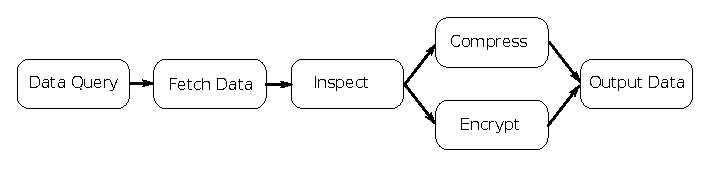
\includegraphics[width=3.5in]{ip-data-proc}
	\label{fig1.1}
}

\subfigure
{
	\includegraphics[width=3in]{op-data-proc}
	\label{fig1.2}
}
\caption{Operations performed on the data stored and retrieved}
\label{fig1}
\end{figure}

The nodes that are connected in the cluster are linked through a switch or router. In such a scenario the number of routers increase with the size of the cluster and the bandwidth required by the application. Due to this the performance of the application is directly dependent on the network especially the functionality of the routers. Moreover with a fixed infrastructure such as this it is not only difficult to upgrade the routers but it would also be a expensive proposition. In such a situation it makes more sense to use software routers which are much more flexible and cheaper and could prove to be a more effective than or in addition to commercial switches or routers.

In implementing the software routers if one were to dedicate several nodes for this purpose it might prove to be inefficient use of resources since the network traffic generated is highly dependent on the applications being executed in such a closed environment. Moreover such systems might act as a communication bottleneck and the routing operations are focused on these nodes. A more effective approach would be to bring the software routers into the nodes that are used for executing the applications itself. In doing this we dedicate a specific set of resources of each node for the packet processing operations and in essence make each node act as a router. All the nodes in such a cluster are connected with each other based on network topology suitable for its requirements. This would make it possible to divide the workload generated due to the network operations across all the nodes in the cluster. In this paper we propose such a system that not only brings the software routers as separate entity into the actual application nodes but takes it a step further and integrates the network operations with the application itself. 

There are several challenges arises due to this mainly how do we tackle such large number of computations both from the application and the network effectively. Two important constraints would enable us to satisfy the requirements posed by such a system. First, the operations of both the application and the network is parallel in nature and second, the presence of co-processors[], network processors[], Graphics Processing Units ( GPUs ) \& General Purpose GPUs ( GPGPUs ) has dramatically improved the capability of commodity hardware. With this theoretically, we should be able to meet the computational demand but if such a system were to succeed an efficient parallel processing engine is crucial.\\

\textit{write a para forward referencing other sections}\\

An important part of our system is the tasks related to packets such as routing, forwarding, etc., Since our design focuses more on the aspects of the parallel framework we utilize the click modular router for the packet processing tasks. Click modular router \cite{click} is a commonly used software router that includes a library of elements which is used in building flexible and reconfigurable routers. It offers a platform that is flexible for rapid development of newer network protocols and achieves good performance. An improved version known as SMP Click \cite{smpclick} also supports thread based parallel processing of network related tasks. Until recently click's performance in the user space was not as good as its kernel space equivalent. This is mainly due to its extensive use of polling driver in the kernel space. Netmap I/O \cite{netmap} provides a set of APIs that could directly access the packets from the NIC and it helped in the recent improvement of click's user space performance. We found the simpler construction of netmap easier to adapt to our framework  compared to other user space packet access APIs.   

Click dynamically constructs routers in which the configuration file is passed as a parameter for the kernel module or user space binary. As a result most of the actual components are dynamically allocated and connected at run time. While this may be an advantage considering the alternate is to recompile the linux kernel, it does act as significant bottleneck in the case of user space. Moreover some of the restrictions on how the configuration can be parallelized limits the actual performance that could be achieved in combination with netmap. By integrating the ability to access click's elements within our parallel processing engine we were able to scale significantly better. This does require a limited amount of modifications to some of click's libraries and elements. In generating the actual code statically, compilers such as gnu c, etc., can perform optimizations such as loop fusions, in-lining, dead code optimization etc., which were not possible previously.

\section{Old Background}

The constant advancement in server hardware has made systems with large number of hardware threads[] readily available. In addition to this the presence of co-processors[], network processors[], Graphics Processing Units ( GPUs ) \& General Purpose GPUs ( GPGPUs ) has dramatically improved the capability of commodity hardware. These developments has paved way to a platform with immense computing potential which existing applications already take advantage of. Along with the improvements in the Multi-Core \& Many-Core processor architecture the memory and I/O speeds have also seen significant improvement. In particular the network subsystem has seen significant growth, in combination with the improvements to optical communication it has lead to 10GbE interfaces being quite common in enterprise servers. While 40GbE and 100GbE are available for backbone infrastructure but would eventually follow into commodity hardware. 

Network applications represent those applications that operate on any of the seven network layers described in the OSI Model. \{describe more here\}

Several previous work have discussed the process of parallelizing network applications[][][] to enable it to run faster in such multi threaded systems. The development of Software routers[][][] is encouraged further because it costs only a fraction of the commodity hardware routers. Moreover the advancements in the network interfaces has made faster interfaces readily in combination with the multi core servers the performance  It has been shown that such routers can be used to process packets at line rate [][][] which has been a challenge on its own. Network applications including those that operate on few or all of the network layers have been designed with sequential processing as the target environment. The shift to multi core architectures in recent times has induced such applications to utilize parallel processing as a alternate means of computing. While this could lead to significant improvement in performance it also suffers from the same problems as any parallel application. These include scalability, load-balancing, data dependency and the presence of non parallel regions in the program apart from those that might arise due to that specific application. The scaling of software routers has been discussed extensively in RouteBricks[] which shows the problems suffered by software routers when they are scaled beyond a single system. One could argue that complexity of network applications such as Deep Packet Inspection ( DPI ), Packet Forwarding, etc., could be handled by a single many socket Multi-Core SMP system. However, as the complexity of network applications develops it would be inevitable but to move to a multi node environment in order to perform the computations and to handle more network bandwidth.

Large scale computing clusters has been used in high-performance scientific application to solve problems and applications of very large size. It uses a cluster of compute nodes and distributes the workload across them in order to solve it faster. These systems utilize parallel programs consisting of both threads and MPI to break massive problems into smaller workload that can be executed in parallel. In addition, the presence of GPUs and GPGPUs requires a mixture of parallelization constructs such as OpenCL, CUDA, etc., in order to achieve the best performance in the system. In this paper we discuss how some of the techniques used by these applications could be used to parallelize network applications.

Click Modular Software Router[] consists of extensive elements which are used to construct software routers. Click primarily targets packet processing applications especially those that operate on L4 - L7. \{elaborate more here\}

Discuss about what each sections contains here.....  

\section{Design}

This section describes the design principles related to our methodology. The objective is to determine the requirements necessary to parallelize network applications. Our methods focus on ways to improve the click system in some cases even extend its functionality.

\subsection{Emphasize on user level execution environment}

The existing software routers are predominantly implemented in the kernel space for the ease of access to resources and can bypass the OS overhead incurred when data is accessed through the network subsystem. While this alternative provides better performance it also leads to concerns regarding stability and security of the system. Newer techniques such as Netmap[] allows direct access to network buffers which makes it possible to write high performance packet processing applications in userspace itself. Typically network applications which operate on L4 - L7 are developed in the kernel space in order to intercept the network packets before it flows through the OS. Whereas those applications that utilize L1 - L3 are present in the user space. The objective here is to completely switch to user space to solve any of the stability or security concerns. In addition, scenarios where the applications that operate across most or all the layers could be improved by combining the operations across the different layers in user space itself.  

\subsection{Eliminate the overhead associated with creation of dynamic objects}

Click constructs application graphs based on dynamic creation of objects and passing the data packets across the virtual functions. Though this is a very elegant approach in creating the software router it does incur the penalty of the virtual function tables. The click-tool[] addresses this issue but it does not solve the problem entirely. The construction of the software router at run time is the primary reason behind it. This mainly arises due to the presence of kernel module which installs the router as a kernel module based on the input configuration. However in the user level it would not be necessary for a separate process to initialize the router instead we could generate the entire program statically including the necessary flow associated with the specific application. This not only eliminates the overhead associated but also opens up means to optimize the graph further. 

\subsection{Optimize based on application graph}

Network applications especially that operate on the lower layers are very sensitive to the overhead associated with operating on the data separately on each layer. Instead given an application graph if we were to provide a sequential flow of the different functions at the various layers then it would be possible for the compiler to optimize the regions of program into a single and optimized block of code. This would also improve the cache locality of the data accessed by consecutive functions. This also presents us with the ability to perform other types of stream graph optimizations[] which would not be possible if the specific graph was constructed dynamically at run time.

\subsection{Automated data parallelism}

Network traffic is a classic example by which data parallelism can be utilized to achieve scalable parallelism. Click's support for parallelism in user level is described as experimental, it is implemented by using a task graph consisting of each work associated with each element which is executed in the threads. The support for parallelism in the kernel mode is better in comparison to that of user mode. Since our target environment is in the user space the proposed design involves a different approach to which we can extract data parallelism. We first split the data across multiple queues and then replicate the application graph across to process the data the queues in parallel. An important condition here is to make sure packets of the same flow should pass through the same queue. Since the application graph can be replicated it also makes it possible to dynamically load balance several applications based on the workload.   

\subsection{Efficient implementation of task parallelism}

In generating the application graph as a sequence of operations it also makes it possible to process different stages of the operation in a pipelined manner. This when combined with stream optimizations and could be used to determine which steps of the graph is best suited to form the stages of a pipeline. The condition to balance here is the weight associated with computation in that stage with that of the overhead incurred in computing the data in two separate stages. It would be necessary to determine whether the additional over head involved in executing the task in parallel provides any significant improvement in performance. 

\section{Implementation}

Click was designed as a means to easily implement a software router on top of a Linux OS. This is implemented in two different ways one is by installing a kernel module and the other is a program that executes in the user level. Both of them accept a configuration file described in click's language specification. This is then used to construct the router by linking the virtual functions for the push and pull operations of the different elements in accordance with the specified graph.

\subsection{Modifications to click system}

\subsubsection{Static Generation Of ???}
The first step in the design was to overcome the limitation of using click's infrastructure to construct the software router which consists of dynamically initialized objects and virtual functions. This was necessary due to two important conditions, one was to eliminate the overhead associated with the dynamic construction of the objects and virtual functions and the other was to provide the compiler a chance to optimize the program during the compilation phase. This would however result in not being able to construct the software router using click's infrastructure but would require the application specific code to be recompiled. This could be a significant hurdle in the case of running the software router in kernel mode where the router configuration is installed by the click kernel module in which case the entire kernel module should be recompiled and reinitialized. Whereas in user space this would not be an issue since routers of different configurations are basically treated as separate applications and would just have to go through an additional compilation phase before being used. The added advantage of this would be to enable network applications that operate on L1 - L3 layers to use the packet processing ( L4 - L7 ) infrastructure provided by click elements.

\subsubsection{Implementation of data parallelism}


--Talk about MPI \& threads\\

--Our goal here is to focus on the network application as a workload and characterize it as such without involving any kind of overhead that might occur due to the network.\\



\section{Experimental Evaluation}

\section{Related Work}

\section{Conclusions}



% An example of a floating figure using the graphicx package.
% Note that \label must occur AFTER (or within) \caption.
% For figures, \caption should occur after the \includegraphics.
% Note that IEEEtran v1.7 and later has special internal code that
% is designed to preserve the operation of \label within \caption
% even when the captionsoff option is in effect. However, because
% of issues like this, it may be the safest practice to put all your
% \label just after \caption rather than within \caption{}.
%
% Reminder: the "draftcls" or "draftclsnofoot", not "draft", class
% option should be used if it is desired that the figures are to be
% displayed while in draft mode.
%
%\begin{figure}[!t]
%\centering
%\includegraphics[width=2.5in]{myfigure}
% where an .eps filename suffix will be assumed under latex, 
% and a .pdf suffix will be assumed for pdflatex; or what has been declared
% via \DeclareGraphicsExtensions.
%\caption{Simulation Results}
%\label{fig_sim}
%\end{figure}

% Note that IEEE typically puts floats only at the top, even when this
% results in a large percentage of a column being occupied by floats.


% An example of a double column floating figure using two subfigures.
% (The subfig.sty package must be loaded for this to work.)
% The subfigure \label commands are set within each subfloat command, the
% \label for the overall figure must come after \caption.
% \hfil must be used as a separator to get equal spacing.
% The subfigure.sty package works much the same way, except \subfigure is
% used instead of \subfloat.
%
%\begin{figure*}[!t]
%\centerline{\subfloat[Case I]\includegraphics[width=2.5in]{subfigcase1}%
%\label{fig_first_case}}
%\hfil
%\subfloat[Case II]{\includegraphics[width=2.5in]{subfigcase2}%
%\label{fig_second_case}}}
%\caption{Simulation results}
%\label{fig_sim}
%\end{figure*}
%
% Note that often IEEE papers with subfigures do not employ subfigure
% captions (using the optional argument to \subfloat), but instead will
% reference/describe all of them (a), (b), etc., within the main caption.


% An example of a floating table. Note that, for IEEE style tables, the 
% \caption command should come BEFORE the table. Table text will default to
% \footnotesize as IEEE normally uses this smaller font for tables.
% The \label must come after \caption as always.
%
%\begin{table}[!t]
%% increase table row spacing, adjust to taste
%\renewcommand{\arraystretch}{1.3}
% if using array.sty, it might be a good idea to tweak the value of
% \extrarowheight as needed to properly center the text within the cells
%\caption{An Example of a Table}
%\label{table_example}
%\centering
%% Some packages, such as MDW tools, offer better commands for making tables
%% than the plain LaTeX2e tabular which is used here.
%\begin{tabular}{|c||c|}
%\hline
%One & Two\\
%\hline
%Three & Four\\
%\hline
%\end{tabular}
%\end{table}


% Note that IEEE does not put floats in the very first column - or typically
% anywhere on the first page for that matter. Also, in-text middle ("here")
% positioning is not used. Most IEEE journals/conferences use top floats
% exclusively. Note that, LaTeX2e, unlike IEEE journals/conferences, places
% footnotes above bottom floats. This can be corrected via the \fnbelowfloat
% command of the stfloats package.

% conference papers do not normally have an appendix


% use section* for acknowledgement
\section*{Acknowledgment}
This work is funded by the IRCSET Enterprise Partnership Scheme along with IBM Research, Ireland.

% trigger a \newpage just before the given reference
% number - used to balance the columns on the last page
% adjust value as needed - may need to be readjusted if
% the document is modified later
%\IEEEtriggeratref{8}
% The "triggered" command can be changed if desired:
%\IEEEtriggercmd{\enlargethispage{-5in}}

% references section

% can use a bibliography generated by BibTeX as a .bbl file
% BibTeX documentation can be easily obtained at:
% http://www.ctan.org/tex-archive/biblio/bibtex/contrib/doc/
% The IEEEtran BibTeX style support page is at:
% http://www.michaelshell.org/tex/ieeetran/bibtex/
%\bibliographystyle{IEEEtran}
% argument is your BibTeX string definitions and bibliography database(s)
%\bibliography{IEEEabrv,../bib/paper}
%
% <OR> manually copy in the resultant .bbl file
% set second argument of \begin to the number of references
% (used to reserve space for the reference number labels box)
%\begin{thebibliography}{1}

%\end{thebibliography}


% that's all folks
\end{document}


